\documentclass{article}
\usepackage[utf8]{inputenc}
\usepackage{graphicx}
\usepackage{amsmath, amssymb, amsfonts}
\usepackage{geometry}
\usepackage{float}
\usepackage{hyperref}
\usepackage{enumitem}
\usepackage{caption}
\usepackage{subcaption}
\usepackage{color}
\usepackage{soul}
\usepackage{listings}
\usepackage{xcolor}
\usepackage{booktabs}

\geometry{a4paper, margin=1in}

\title{Methods in Computational Neuroscience:\\The Neural Code: Spike Train Statistics}
\author{[Sepehr Saeedpour]}
\date{\today}

\begin{document}

\maketitle

% \begin{abstract}
% This report presents a comprehensive analysis of spike train statistics in computational neuroscience. We examine synthetic spike trains generated through Poisson processes and analyze real neuronal data from a monkey's primary somatosensory cortex during vibratory fingertip stimulation. The analysis includes spike train generation, raster plot visualization, inter-spike interval distributions, and the relationship between neuronal firing rates and stimulus frequencies. The results demonstrate how neurons encode information through specific firing patterns and reveal the tuning properties of sensory neurons to different stimulus parameters.
% \end{abstract}

\section*{Introduction}

The study of neural coding has a rich history in neuroscience, beginning with early research on how neurons communicate sensory information through patterns of electrical activity, known as spike trains. In the 1920s, Edgar Adrian and Yngve Zotterman discovered that neurons increased their firing rates when a stimulus, like a weight, became heavier. Their work established the principle of rate coding, where stimulus strength is represented by how fast neurons fire. Over time, research has expanded beyond just firing rates to explore how the timing and synchronization of spikes can also convey information. Modern computational neuroscience now uses detailed statistical methods to analyze spike train data, improving our understanding of how neurons represent sensory information. 

This report specifically investigates spike trains by creating synthetic data using Poisson processes, and analyzing actual neural responses recorded from a monkey’s primary somatosensory cortex when experiencing tactile vibrations.

% The  brain’s  ability  to  process  and  transmit  information  relies  on  the  generation  of  action  potentials,or  spikes,  by  individual  neurons.   These  spikes  form  temporal  patterns  known  as  spike  trains,  whichconstitute the primary language of neural communication.  Understanding how information is encodedin these spike trains is a fundamental challenge in computational neuroscience.In this report, we investigate spike train statistics through both computational modeling and analysisof real neurophysiological data. We begin by generating synthetic spike trains following Poisson statistics,a common model for neuronal firing patterns.  We then analyze the statistical properties of these spiketrains, including their count distributions and inter-spike intervals.  Finally, we examine real neuronaldata recorded from a monkey’s primary somatosensory cortex during vibratory stimulation, investigatinghow neurons encode stimulus frequency through their firing patterns.Through this analysis, we aim to provide insights into the neural code—the set of principles by whichneurons represent and transmit information through spike patterns.  By understanding these principles,we can build better models of neural processing and gain deeper insights into how the brain processessensory information.

\section{Spike Train Statistics}

\subsection{Create a Spike Train}

For a Poisson process with rate $\lambda$, the probability of a spike occurring in a small time interval $\Delta t$ is:

\begin{equation}
    P(\text{spike in interval } \Delta t) = \lambda \Delta t
\end{equation}

A spike train is generated with a length of 1 second and an average rate of 250 spikes per second, using time bins of 1 millisecond ($\Delta t = 1$ ms), resulting in 1000 time bins total.

To generate this Poisson spike train, I defined parameters duration $T = 1$ second, time bin $\Delta t = 0.001$ seconds, and firing rate $\lambda = 250$ Hz.
For each time bin, generated a random number $r$ from a uniform distribution between 0 and 1 and if $r < \lambda \Delta t$, assign a spike (1) to that bin; otherwise, assign no spike (0).



\begin{figure}[H]
\centering
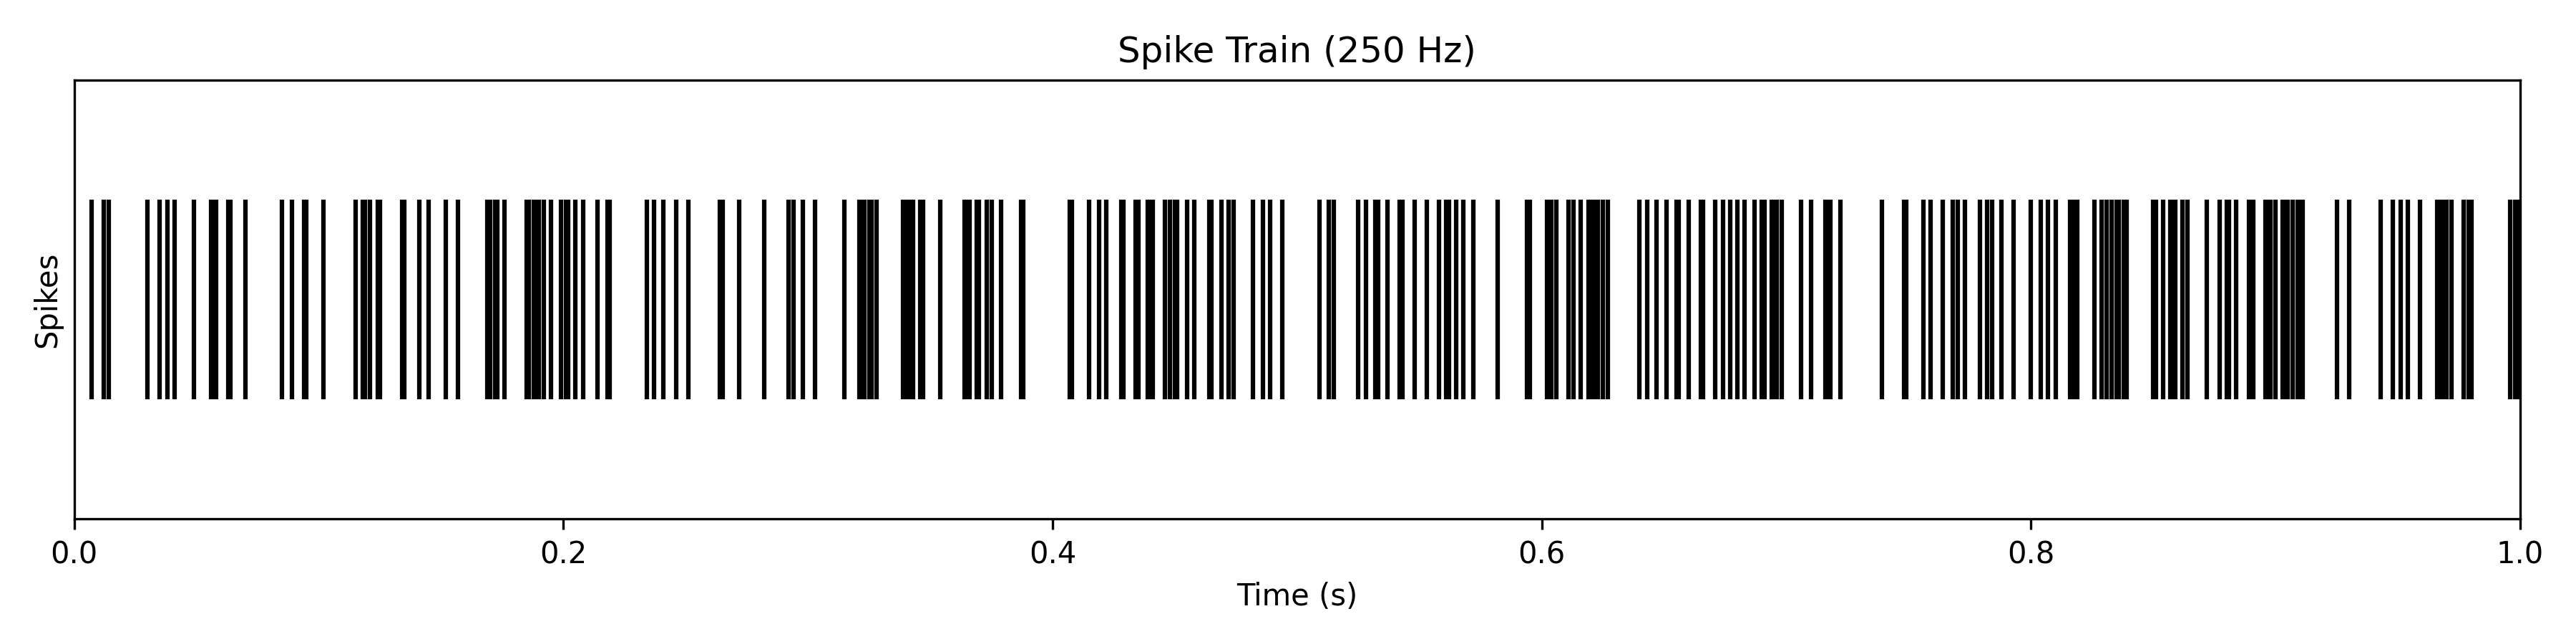
\includegraphics[width=0.8\textwidth]{Fig1.png}
\caption{Spike train with firing rate of 250 Hz. Each vertical line represents a spike, and their distribution follows a Poisson process.}
\label{fig:spike_train}
\end{figure}

The spike train shows the expected statistical properties of a Poisson process, with approximately 250 spikes randomly distributed throughout the 1-second interval. The spike times appear irregular and independent, consistent with the Poisson process's defining characteristics.

\subsection{Create a Raster Plot and Compute the Spike Counts}

$N = 300$ spike trains are generated with a firing rate of 80 Hz and counted the total number of spikes in each train.


\
For a Poisson process with rate $\lambda = 80$ Hz over a period $T = 1$ second, the number of spikes follows a Poisson distribution:
\begin{equation}
    P(k \text{ spikes}) = \frac{(\lambda T)^k e^{-\lambda T}}{k!}
\end{equation}

With mean and variance both equal to $\lambda T = 80$.

\begin{figure}[H]
\centering
\begin{subfigure}{0.48\textwidth}
    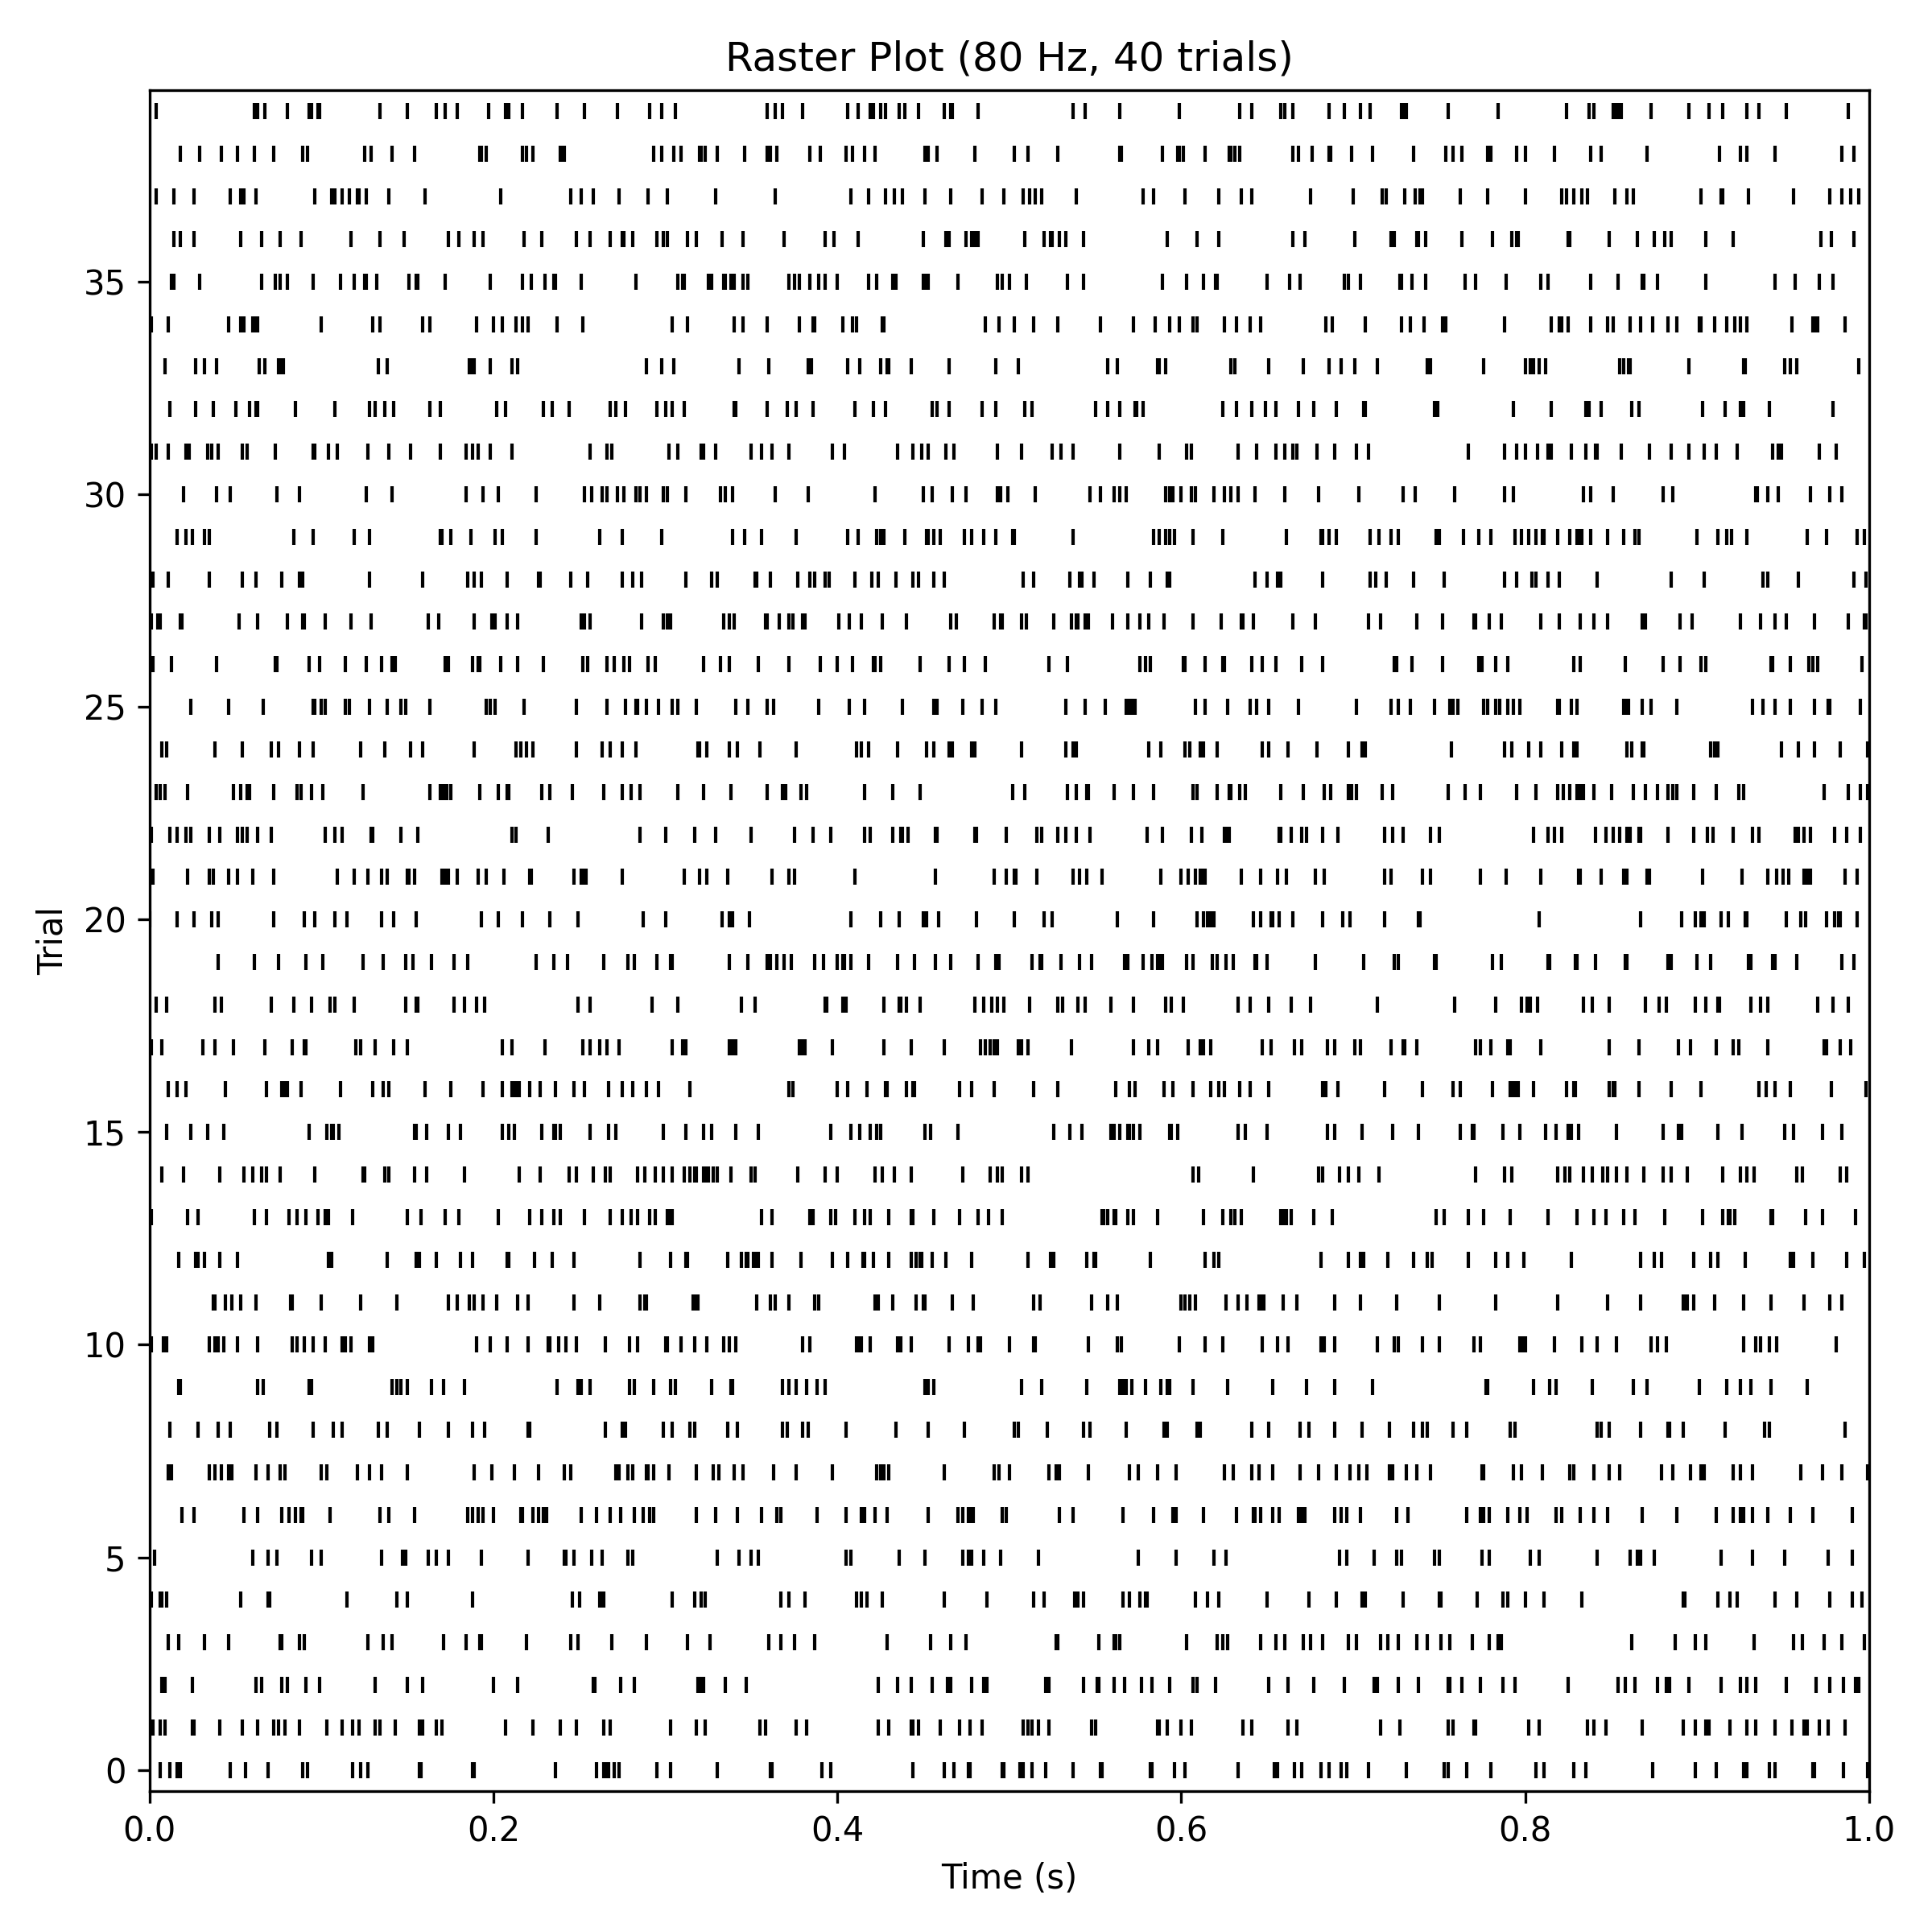
\includegraphics[width=\textwidth]{Fig2a.png}
    \caption{Raster plot showing 40 spike trains with firing rate of 80 Hz. Each row represents one trial, and each vertical line represents a spike.}
    \label{fig:raster_plot}
\end{subfigure}
\hfill
\begin{subfigure}{0.48\textwidth}
    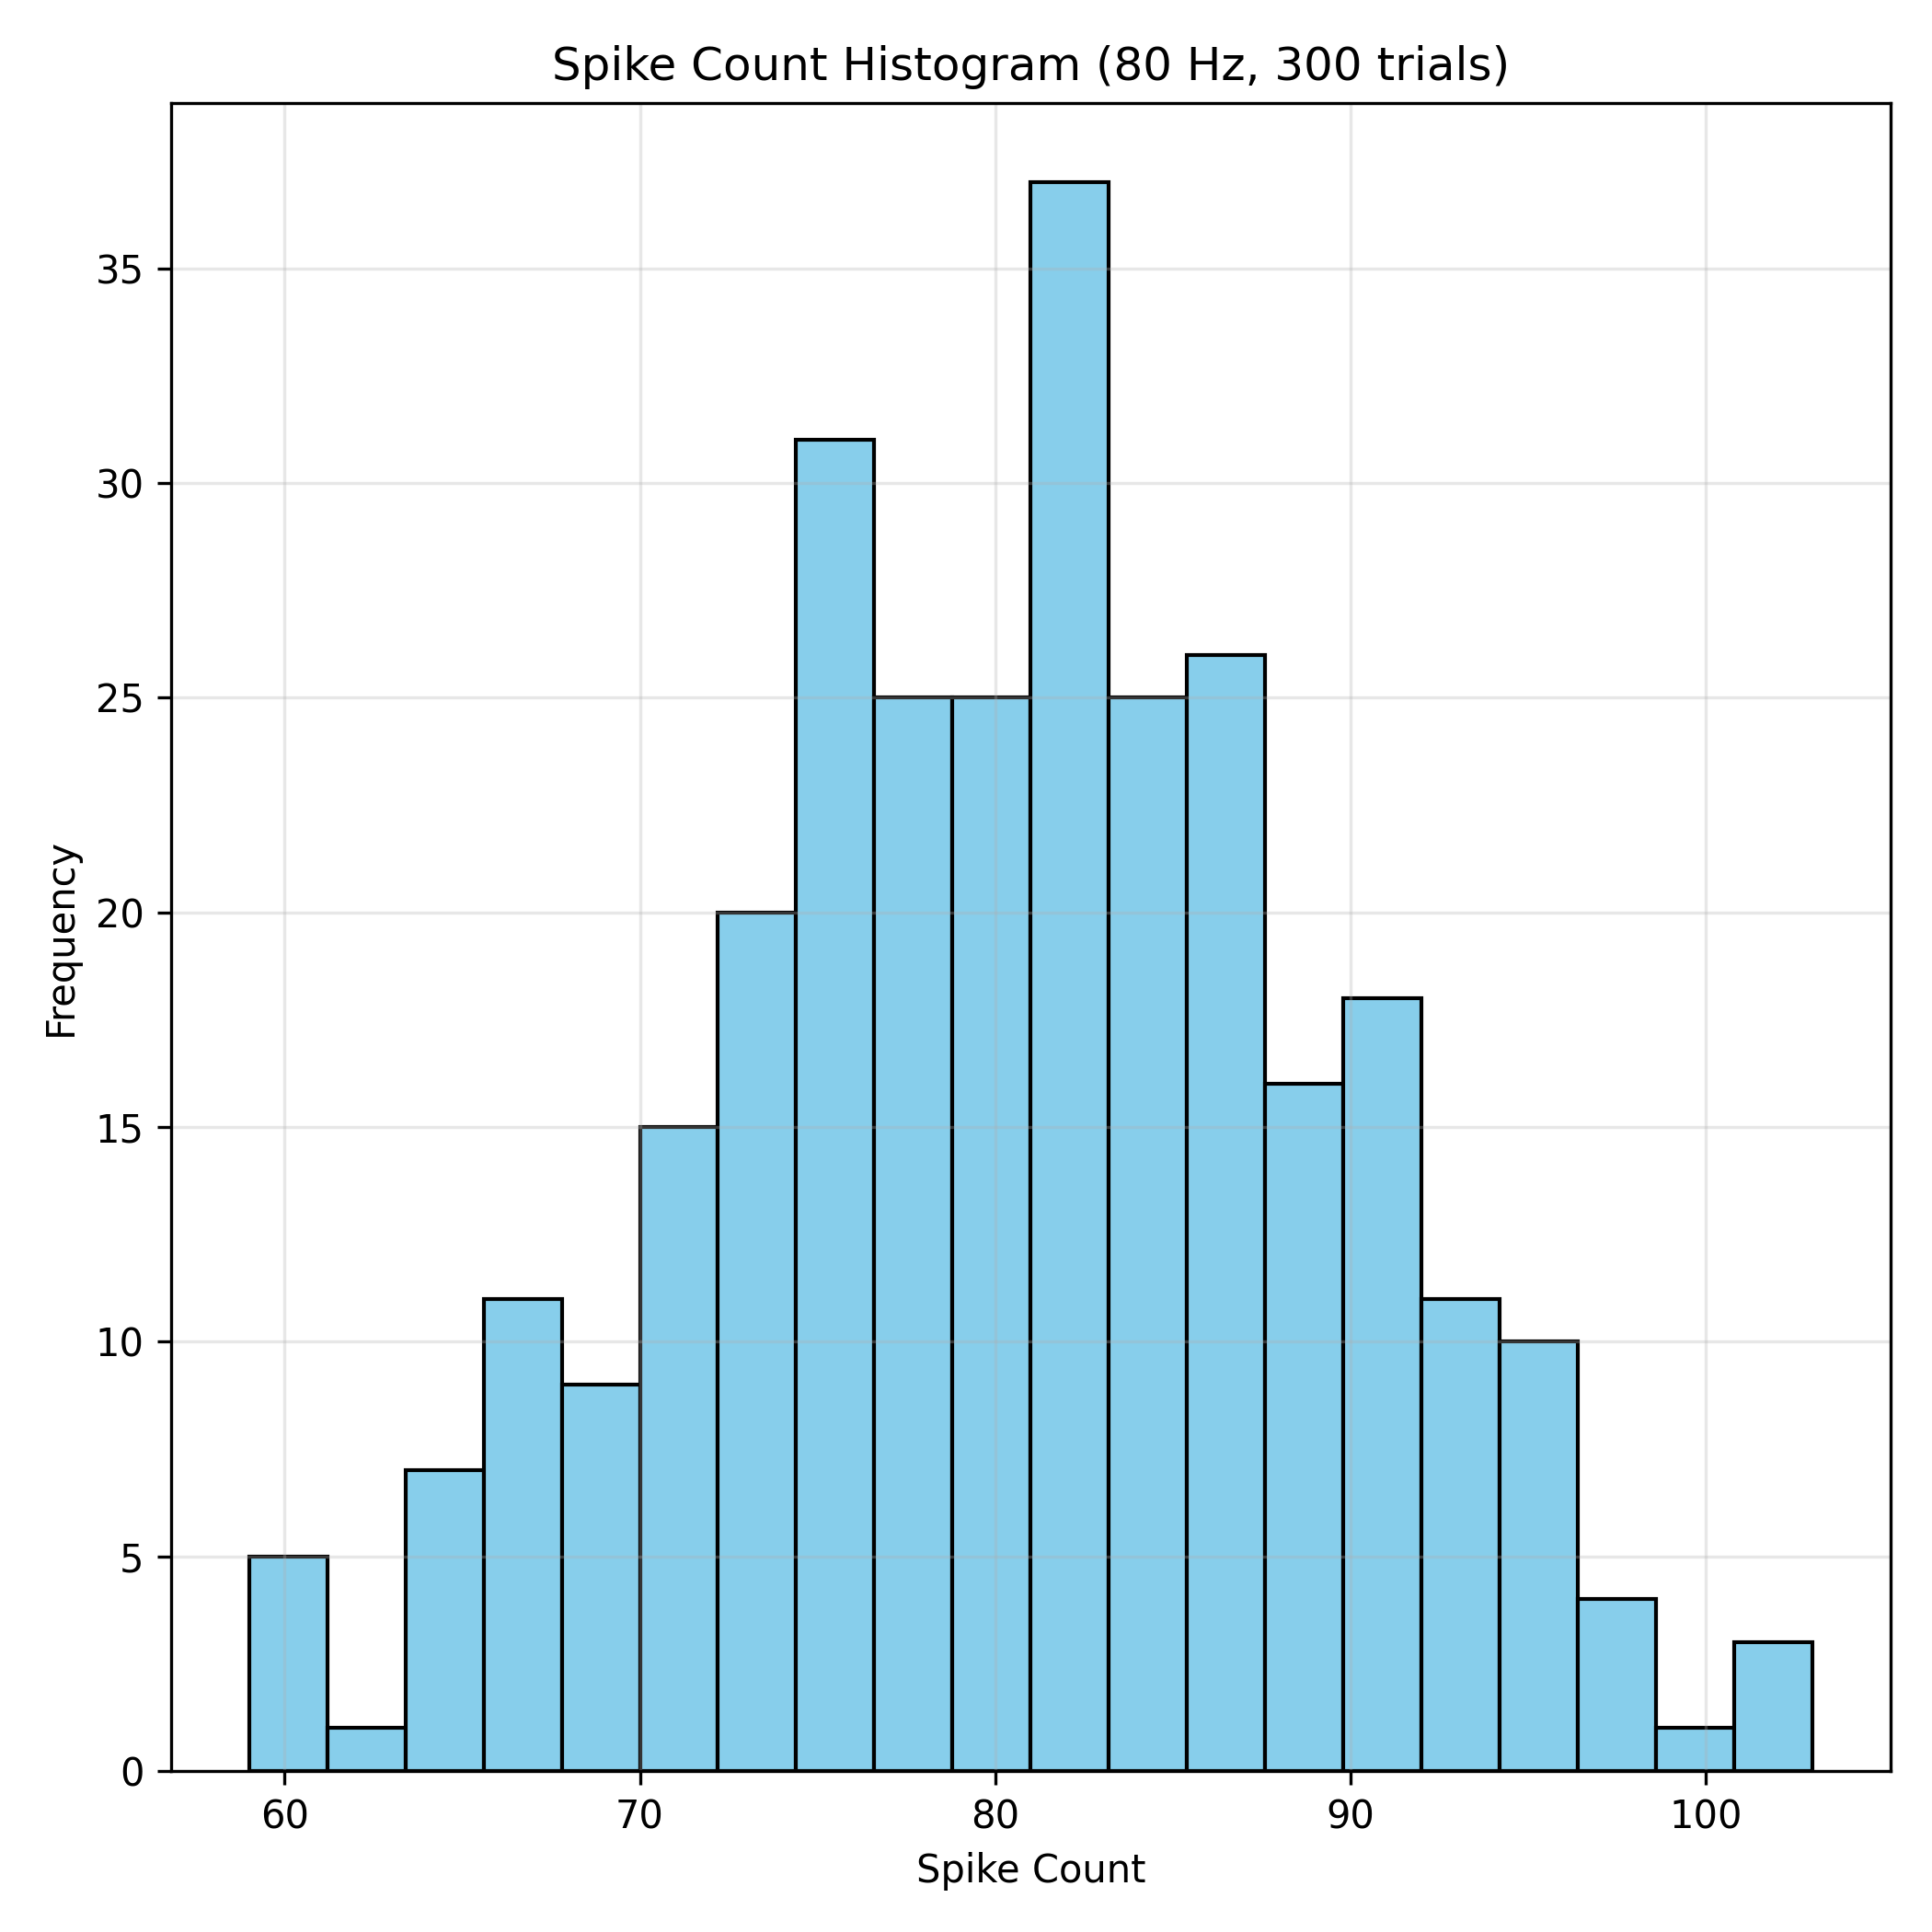
\includegraphics[width=\textwidth]{Fig2b.png}
    \caption{Histogram of spike counts across 300 trials with firing rate of 80 Hz. The red curve shows the theoretical Poisson distribution with mean $\lambda = 80$.}
    \label{fig:spike_count_hist}
\end{subfigure}
\caption{Raster plot and spike count distribution for synthetic spike trains.}
\end{figure}

\begin{itemize}
\item Mean spike count: 80.97 $\approx$ 80 (mathces theoretical expectation)
\item Variance of spike counts: 80.16 $\approx$ 80 (matches theoretical expectation)
\end{itemize}


The close agreement between the mean and variance, and the histogram's shape matching the theoretical Poisson distribution, confirms that our spike generator correctly implements a Poisson process. 
The raster plot visually demonstrates the randomness and independence of spike times across trials, which are fundamental properties of the Poisson process.

\subsection{Inter-Spike Interval Distribution}

The histogram of inter-spike intervals (ISIs) is computed for the spike trains generated in 1.2 and so is the Coefficient of Variation (CV).

For a Poisson process with rate $\lambda$, the ISI follows an exponential distribution:
\begin{equation}
    P(ISI = t) = \lambda e^{-\lambda t}
\end{equation}

With ISI mean = $1/\lambda = 1/80 = 0.0125$ seconds (12.5 ms) and ISI standard deviation also equal to $1/\lambda = 0.0125$.

The Coefficient of Variation (CV) is defined as:
\begin{equation}
    CV = \frac{\sigma_{ISI}}{E[ISI]}
\end{equation}

For a Poisson process, $CV = 1$ because the standard deviation equals the mean.

\begin{figure}[H]
\centering
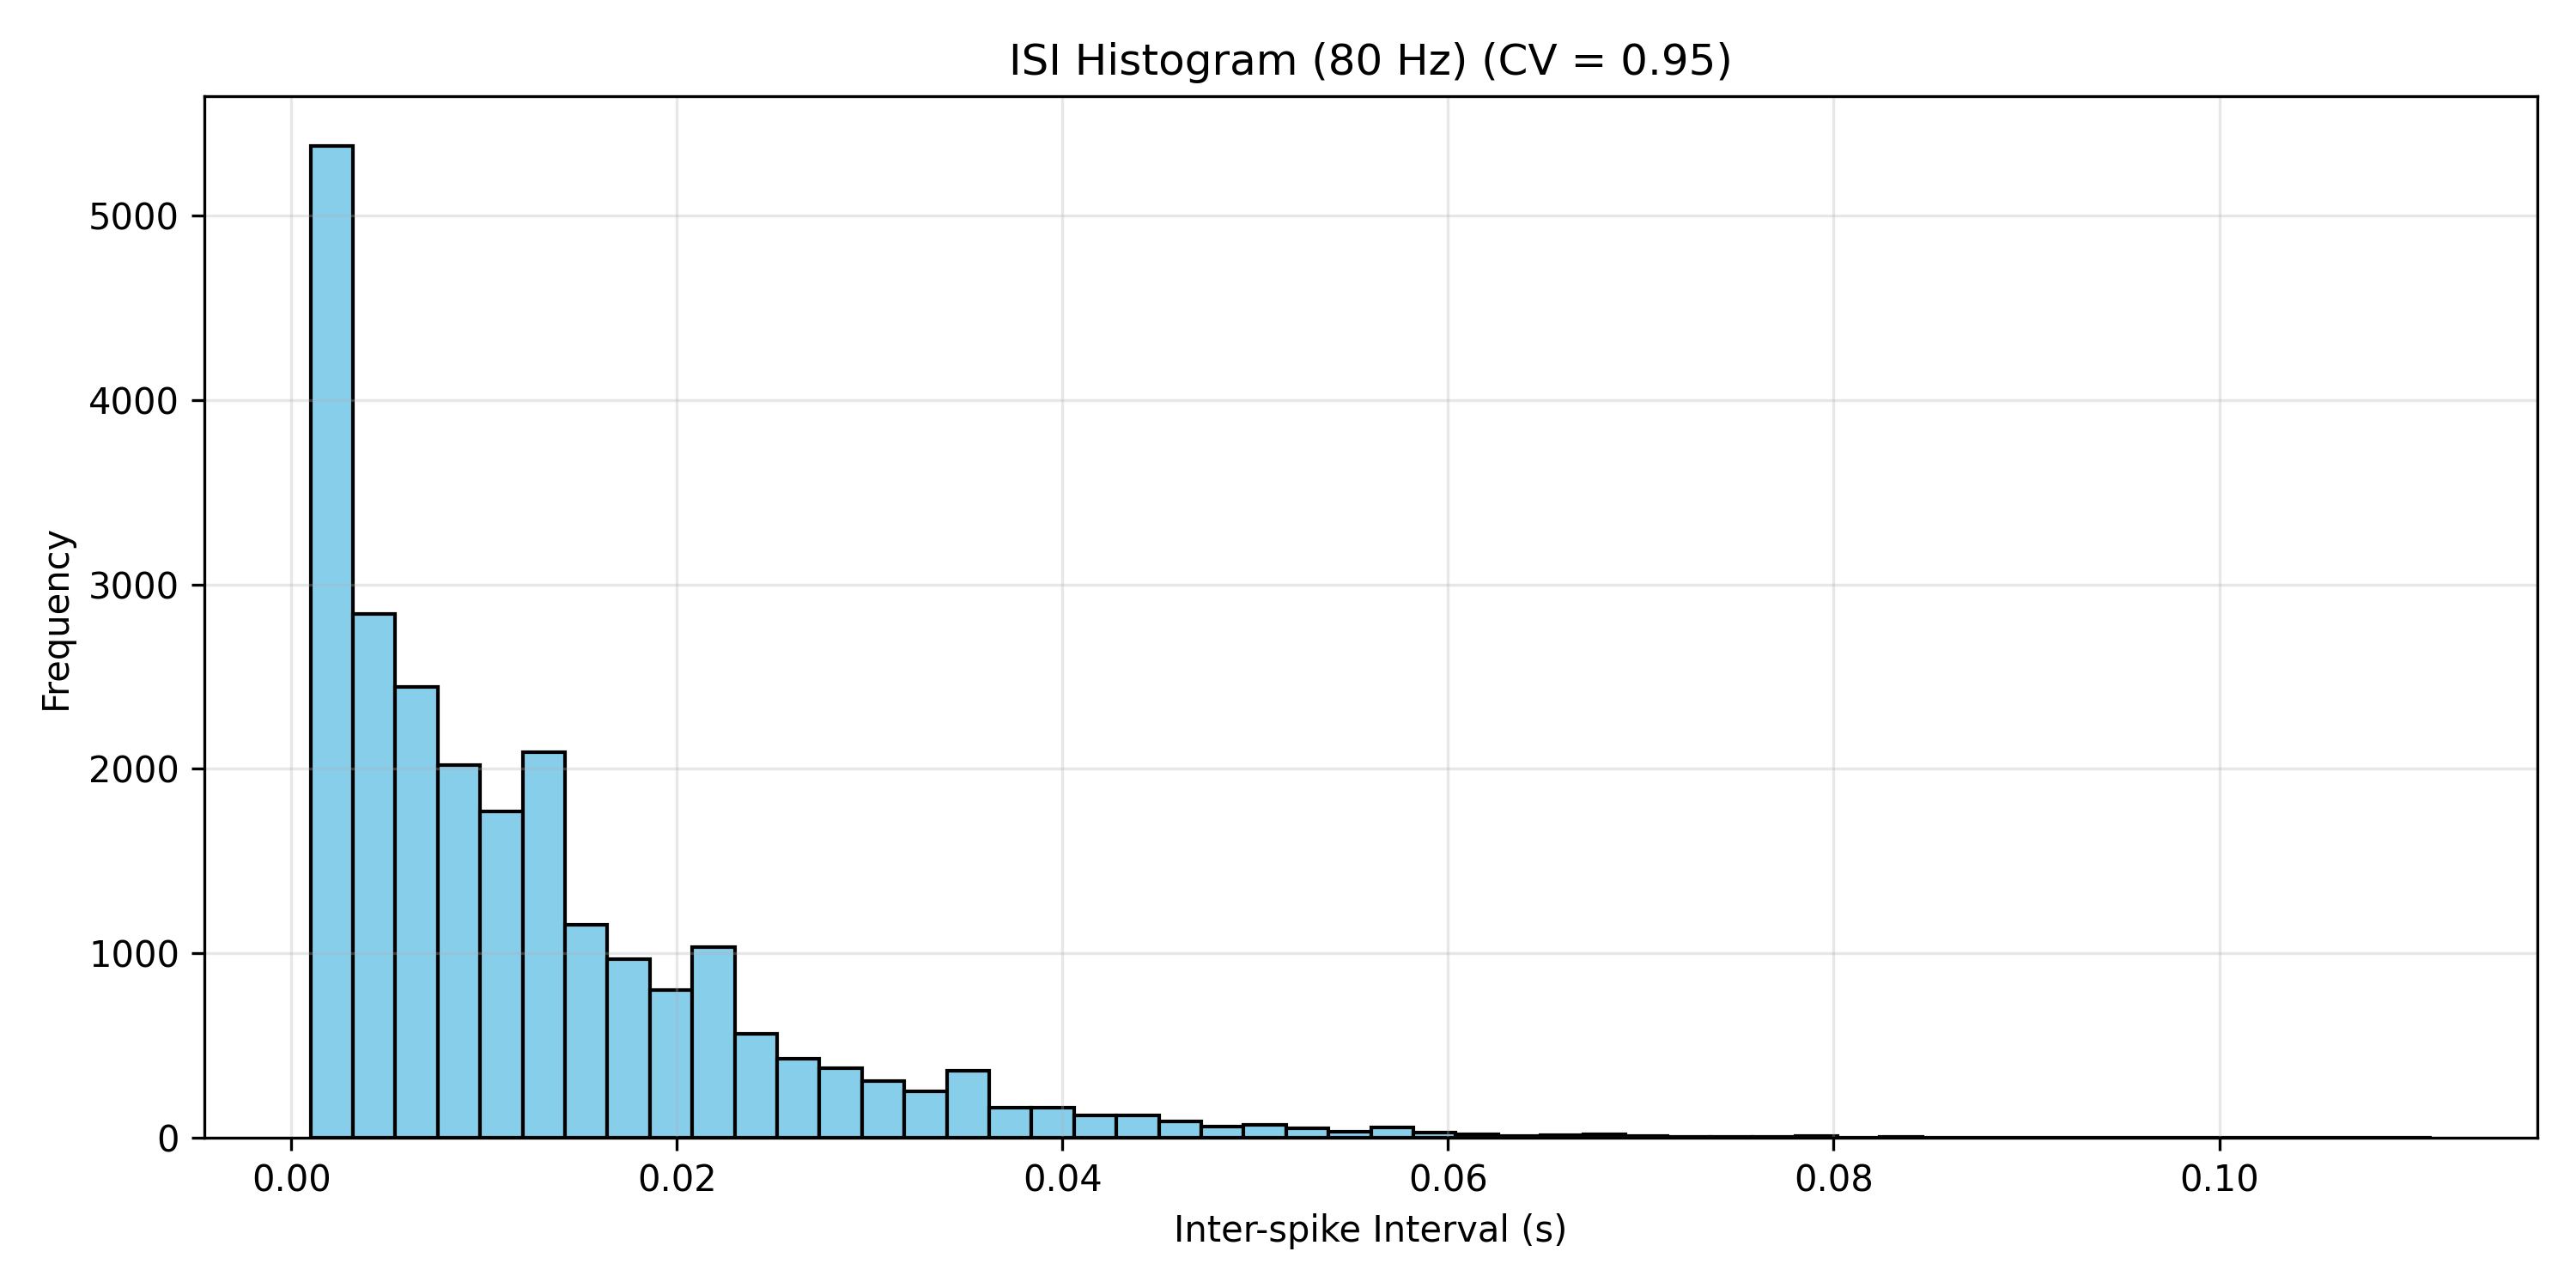
\includegraphics[width=0.7\textwidth]{Fig3.png}
\caption{Histogram of inter-spike intervals for spike trains with firing rate of 80 Hz.}
\label{fig:isi_hist}
\end{figure}

% \subsubsection*{Analysis:}
\begin{itemize}
    \item Mean ISI: 12.28 ms $\approx$ 12.5 ms (theoretical expectation)
    \item Standard deviation of ISI: 11.62 ms $\approx$ 12.5 ms (theoretical expectation)
    \item Coefficient of Variation (CV): 0.95 $\approx$ 1.0 (theoretical expectation)
\end{itemize}

% \subsubsection*{Interpretation of CV:}
The CV value of approximately 1 indicates that the spike trains exhibit the irregular firing pattern characteristic of a Poisson process. 
This value means that the standard deviation of the ISIs is nearly equal to the mean, which is expected for exponentially distributed intervals. 

In neuronal recordings:
\begin{itemize}
    \item CV $\approx$ 1: Irregular, Poisson-like firing (common in cortical neurons during spontaneous activity)
    \item CV $<$ 1: More regular firing than a Poisson process (seen in some sensory neurons or pacemaker cells)
    \item CV $>$ 1: More irregular or "bursty" firing than a Poisson process (clusters of spikes followed by longer silent periods)
\end{itemize}

Our CV of 0.95 confirms that our synthetic spike trains successfully model the irregular firing statistics seen in many cortical neurons.

\section{Analysis of Real Spike Trains}

\subsection{Raster Plot}

Spike trains recorded from a neuron in the primary somatosensory cortex of a monkey during vibratory fingertip stimulation are analyzed. First, the response to the lowest stimulus frequency (8.4 Hz) is examined.

\begin{figure}[H]
\centering
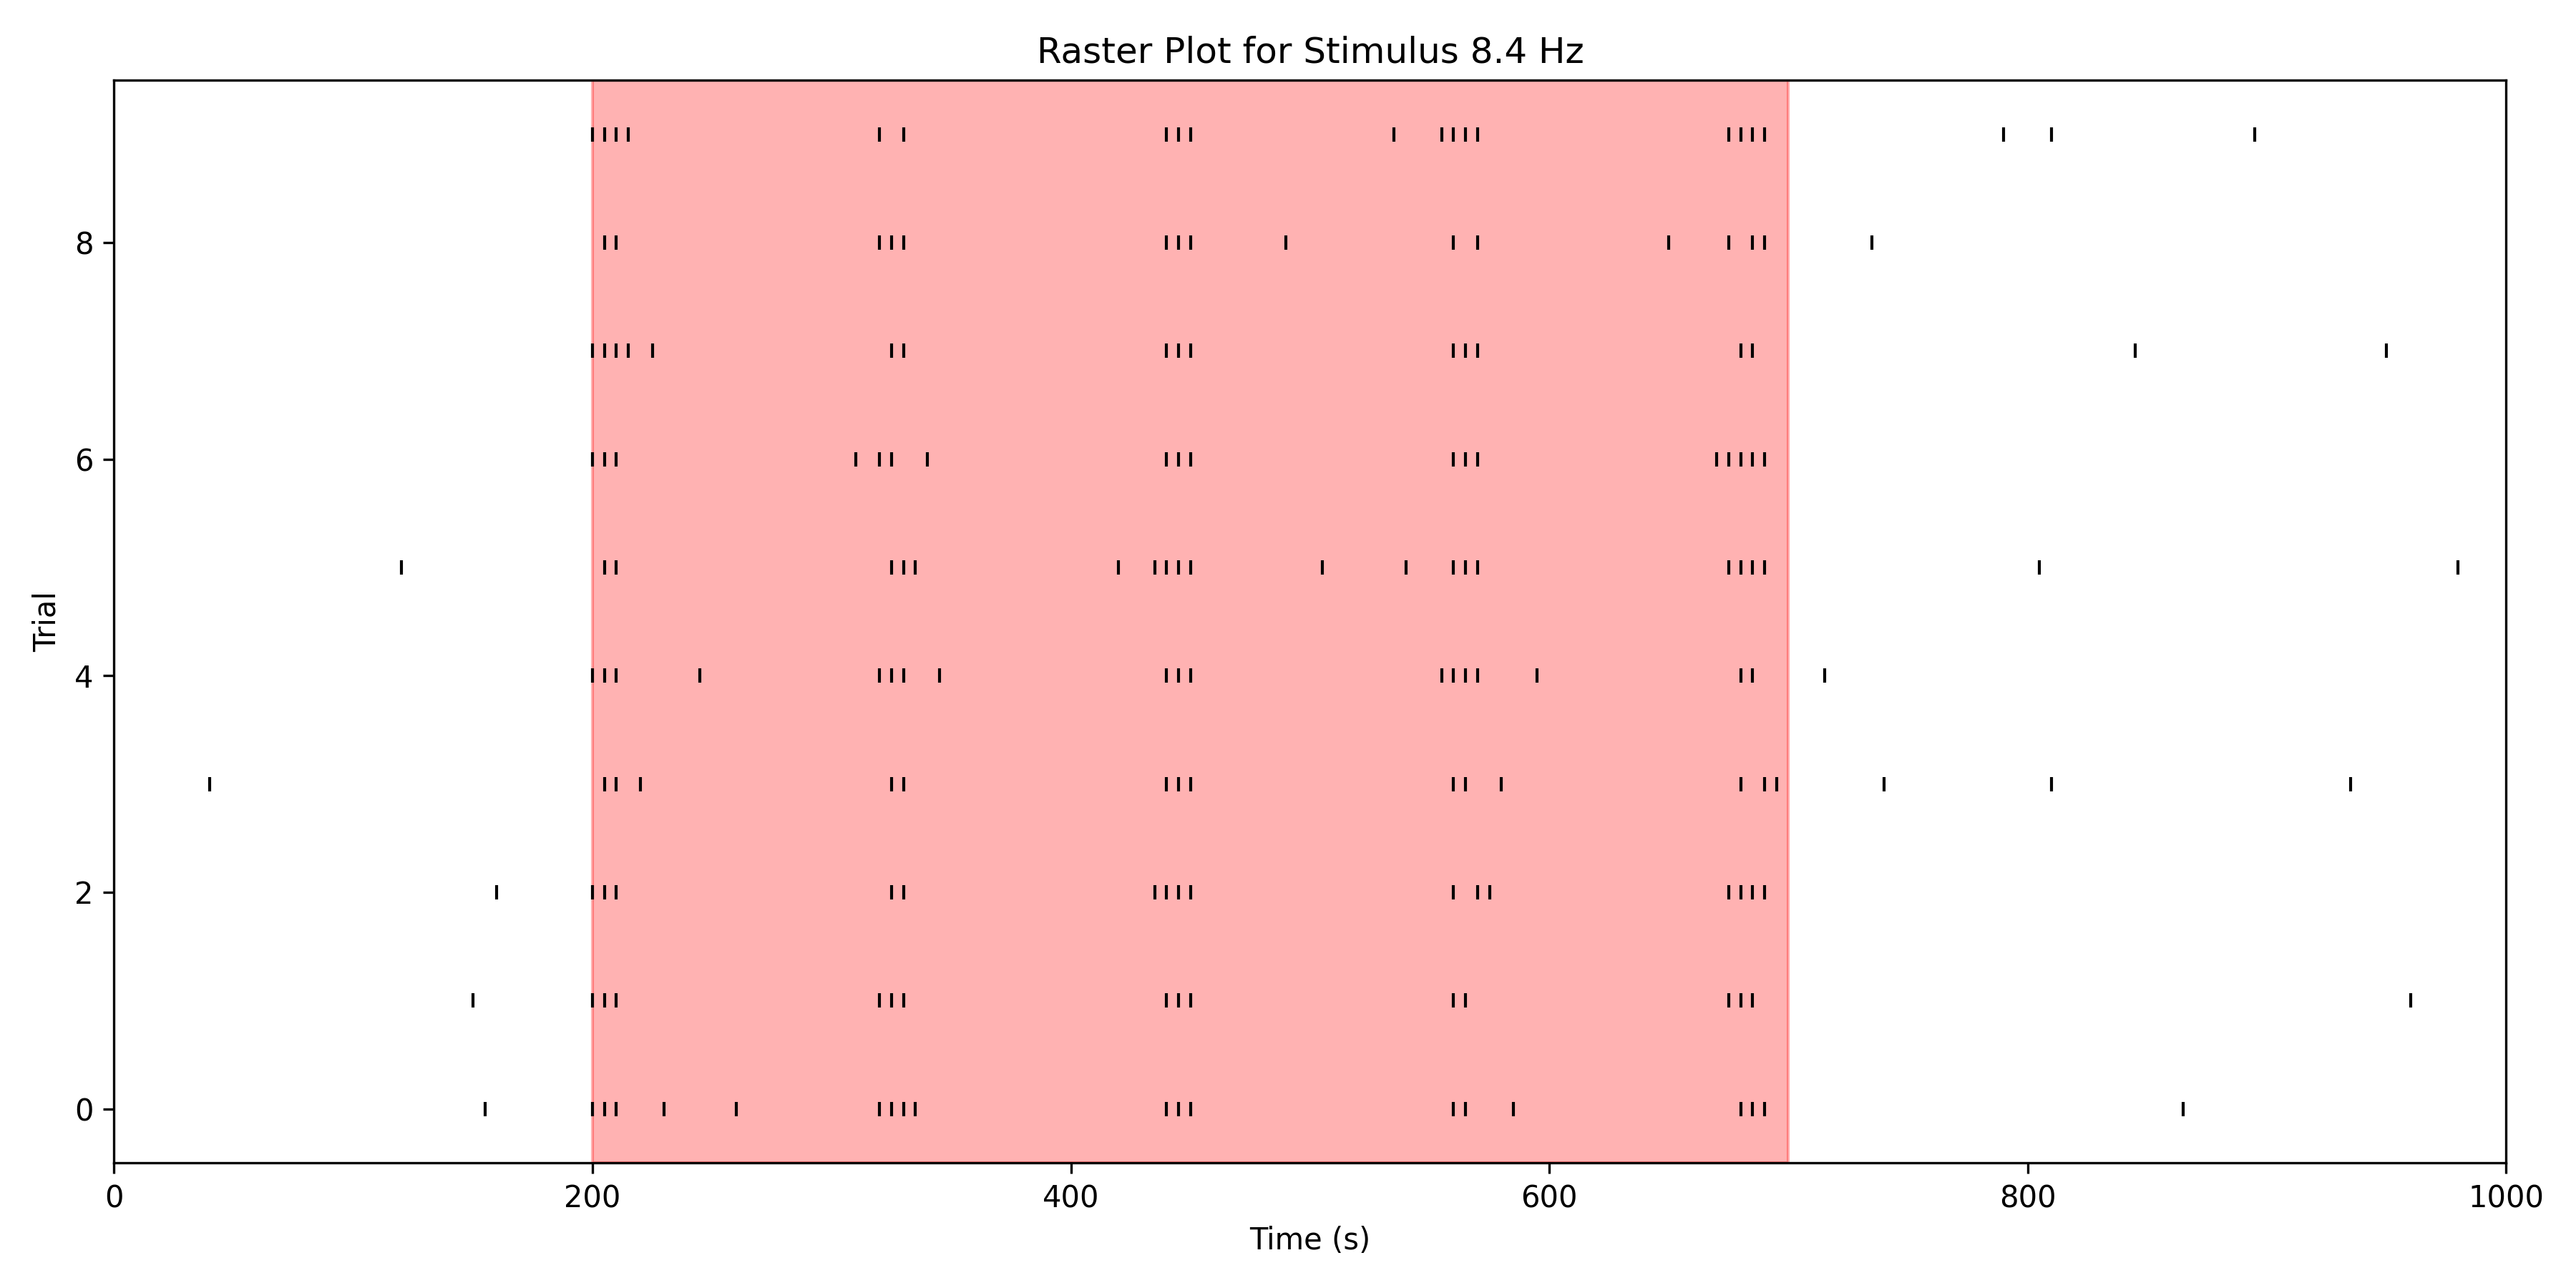
\includegraphics[width=0.8\textwidth]{Fig4_8.4Hz.png}
\caption{Raster plot for neuronal responses to 8.4 Hz vibratory stimulus. The red shaded area indicates the stimulation period (200-700 ms).}
\label{fig:real_raster}
\end{figure}

There is a clear increase in firing rate during the stimulation period (200-700 ms). The neuron exhibits some spontaneous activity before and after stimulation.
Also, there is trial-to-trial variability in the precise timing of spikes. 


This raster plot provides initial evidence that the neuron is responsive to the vibratory stimulus, as indicated by the increased density of spikes during the stimulation period.

\subsection{Spike Count: Mean and Variance}

The number of spikes in each trial during the stimulation period (200-700 ms) for the 8.4 Hz stimulus condition is counter.


\begin{table}[H]
\centering
\begin{tabular}{lc}
\toprule
\textbf{Statistical Measure} & \textbf{Value} \\
\midrule
Mean spike count    & 16.50 spikes/trial \\
Variance            & 3.25 \\
Mean firing rate    & 33.0 spikes/second \\
\bottomrule
\end{tabular}
\caption{Spike count statistics for the 8.4 Hz stimulus condition.}
\label{tab:spike_count_stats}
\end{table}

The variance (3.25) is much smaller than the mean (16.50), indicating a significant deviation from pure Poisson statistics. 
In a Poisson process, the variance would equal the mean but this sub-Poisson variability suggests more regular and importantly, stimulus-driven regularization of the firing pattern.


The mean firing rate of 33.0 spikes/second during stimulation represents a substantial increase from the baseline (pre-stimulus) rate, confirming the neuron's responsiveness to the vibratory stimulus. The sub-Poisson statistics suggest that the neuron's response to this stimulus is not only increased in rate but also more precisely timed than would be expected from a purely random process.

\subsection{Spike Density}

The spike density function is calculated during the stimulation period to visualize the temporal profile of the neuron's response to the 8.4 Hz stimulus.

The spike density function represents the instantaneous firing rate as a function of time, calculated as:
\begin{equation}
    \text{Spike Density}(t) = \frac{\text{Number of spikes at time } t \text{ across all trials}}{\text{Number of trials} \times \Delta t}
\end{equation}


\begin{figure}[H]
\centering
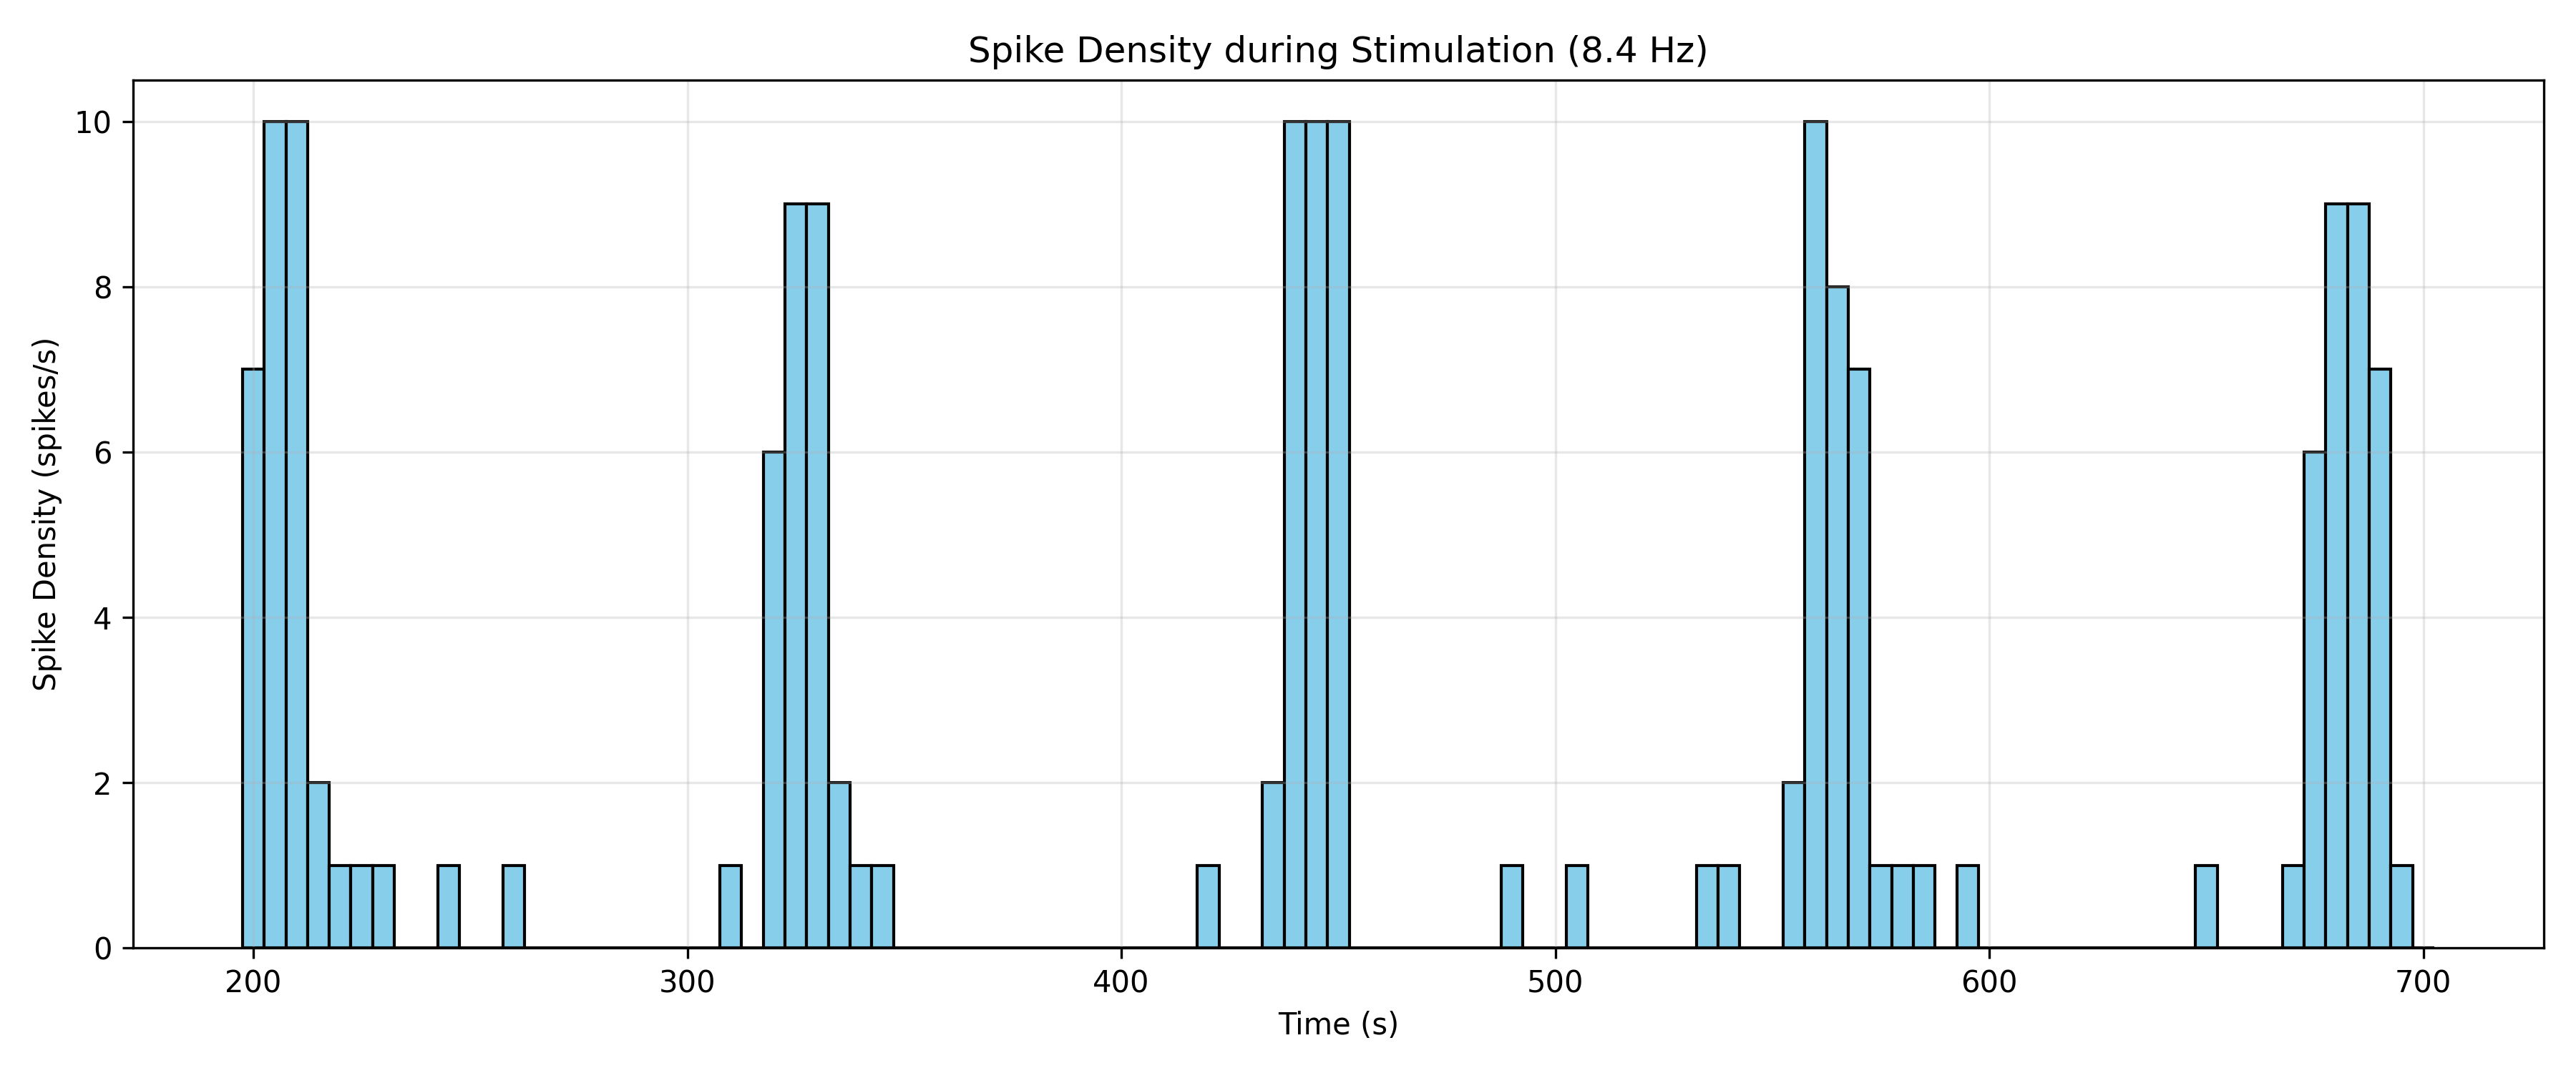
\includegraphics[width=0.8\textwidth]{Fig5.png}
\caption{Spike density during stimulation for 8.4 Hz vibratory stimulus. The plot shows the instantaneous firing rate as a function of time.}
\label{fig:spike_density}
\end{figure}

There is a rapid increase in firing rate at stimulus onset (200 ms) and a subtle oscillations in firing rate that is possibly related to the stimulus cycling at 8.4 Hz.
   
The spike density function provides a more detailed view of the temporal dynamics of the neuron's response than can be observed in the raster plot alone.

\subsection{All Raster Plots Together}

Raster plots for all eight stimulus frequencies are generated and visualized together to compare the neuronal responses across different vibration frequencies.


\begin{figure}[H]
\centering
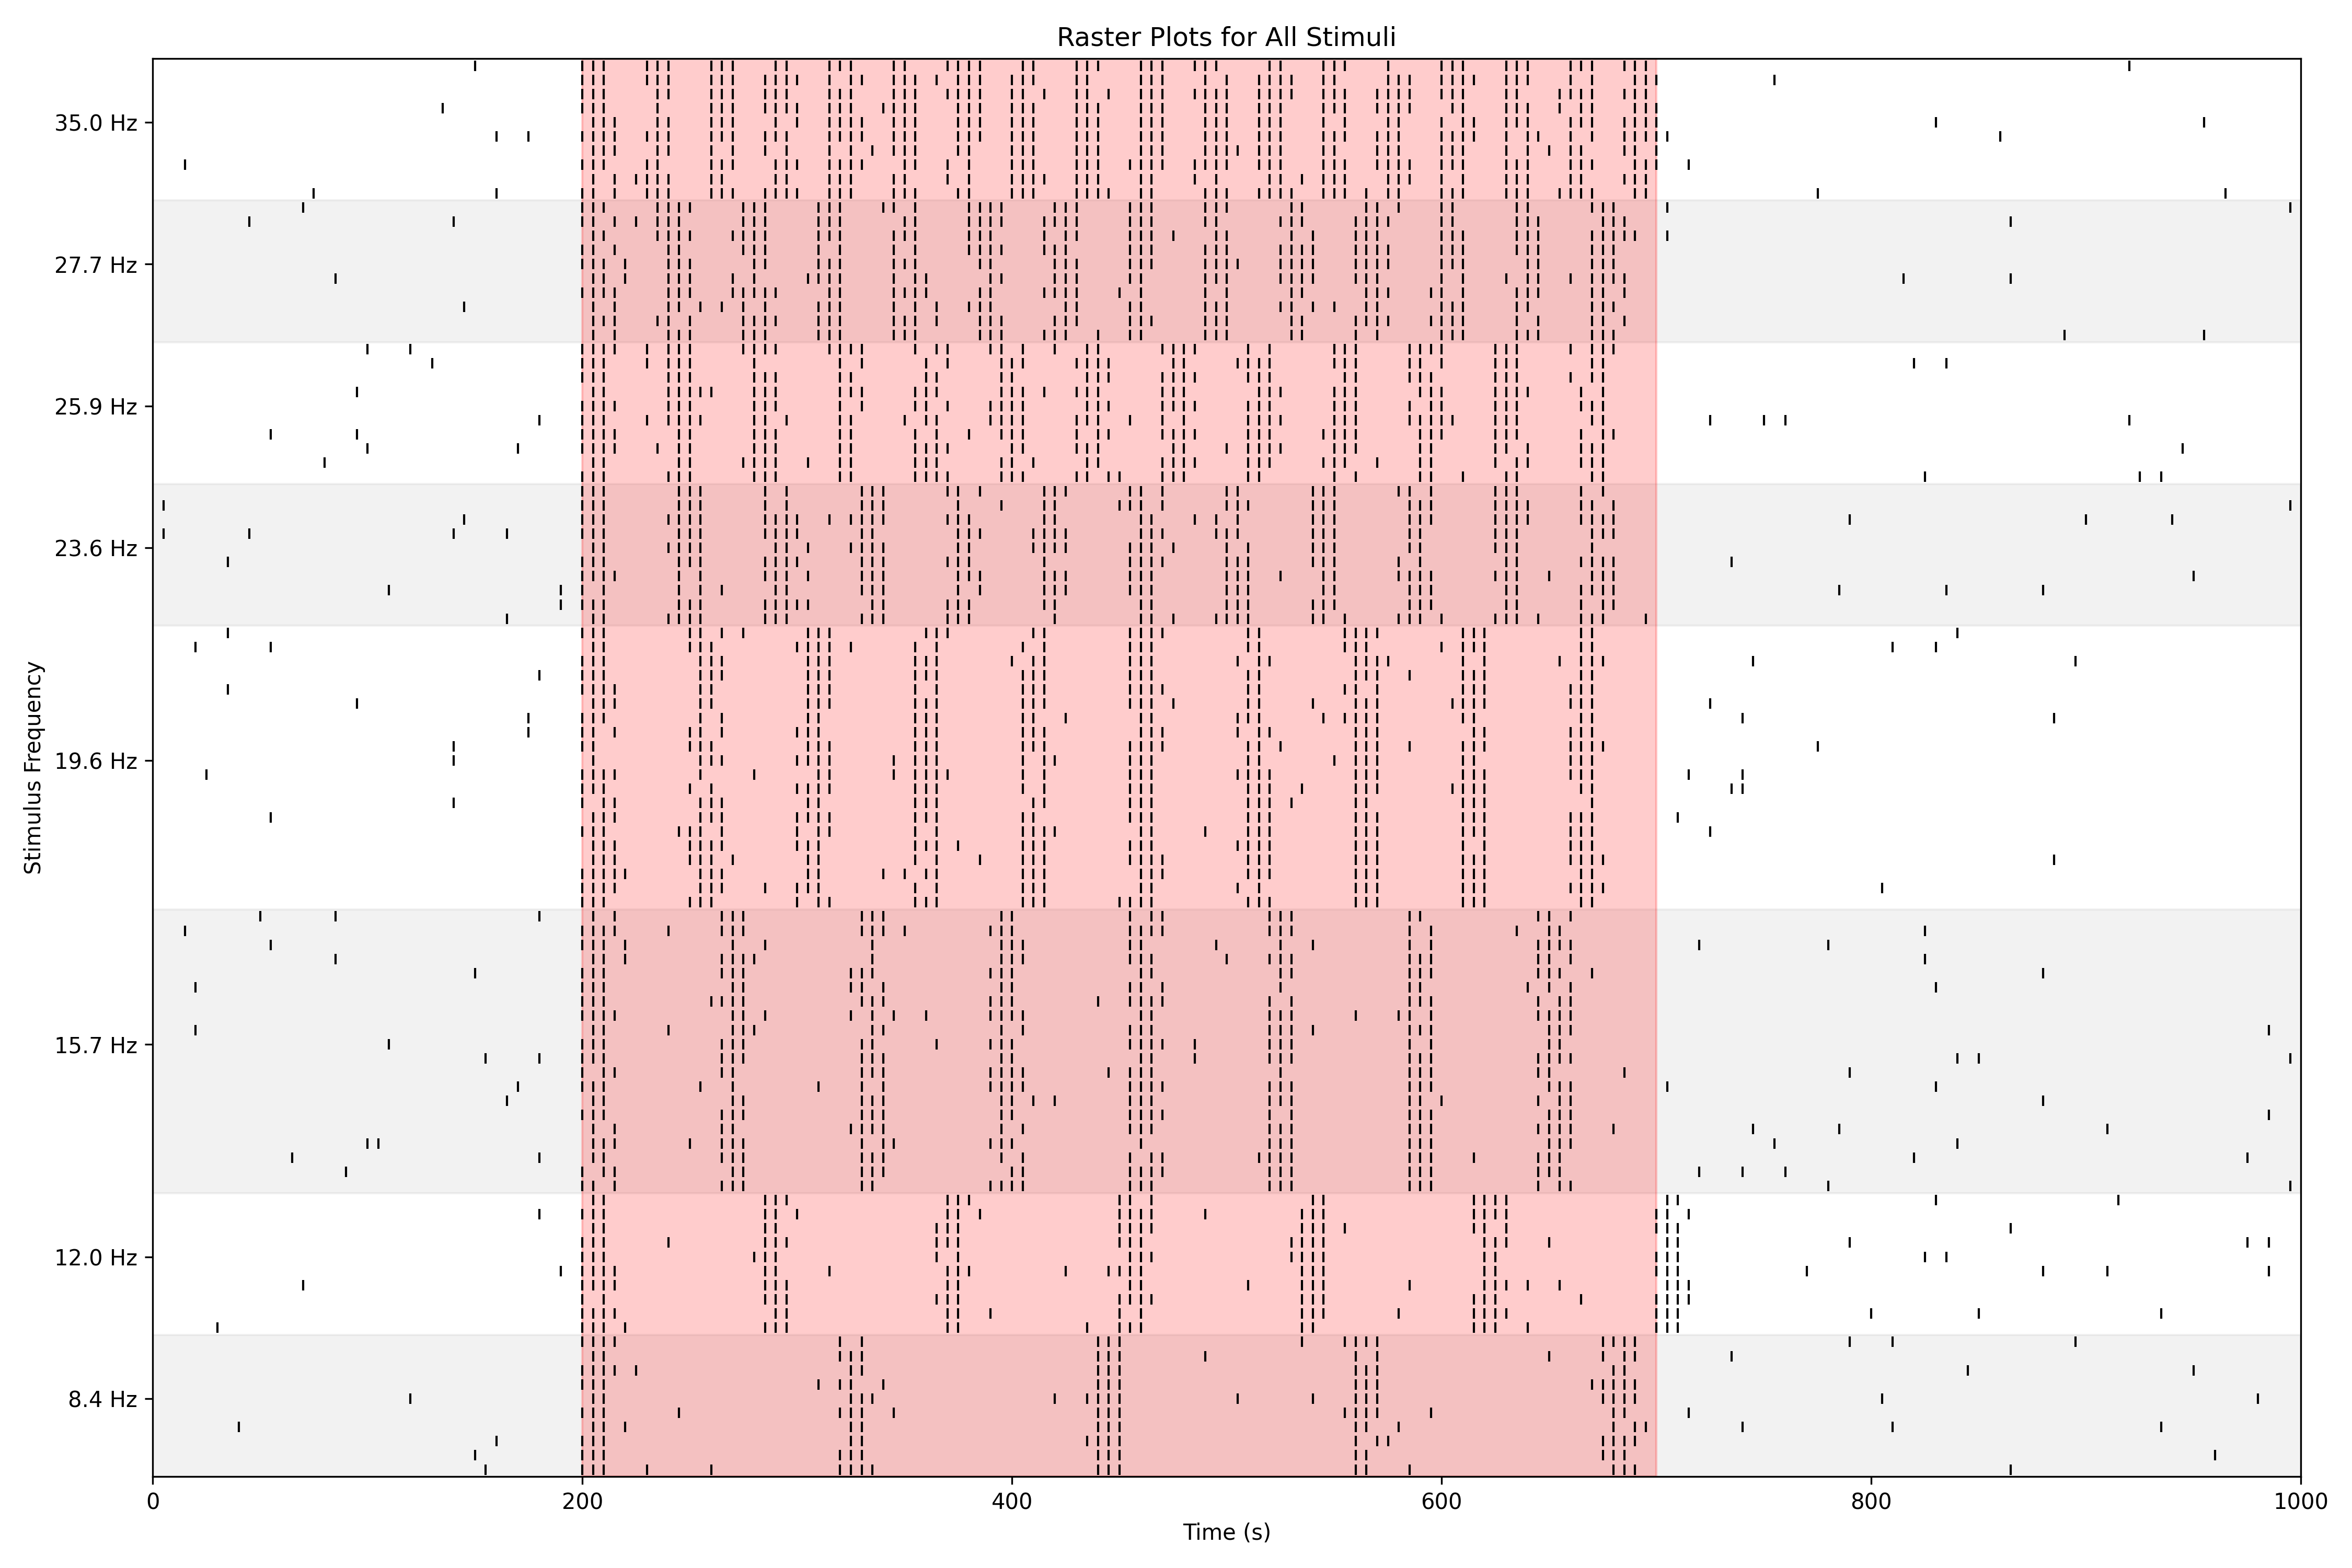
\includegraphics[width=0.9\textwidth]{Fig6.png}
\caption{Combined raster plots for all stimulus frequencies. Different background shading indicates different stimulus frequencies, and the red shaded area indicates the stimulation period (200-700 ms).}
\label{fig:all_rasters}
\end{figure}

\begin{figure}[H]
\centering
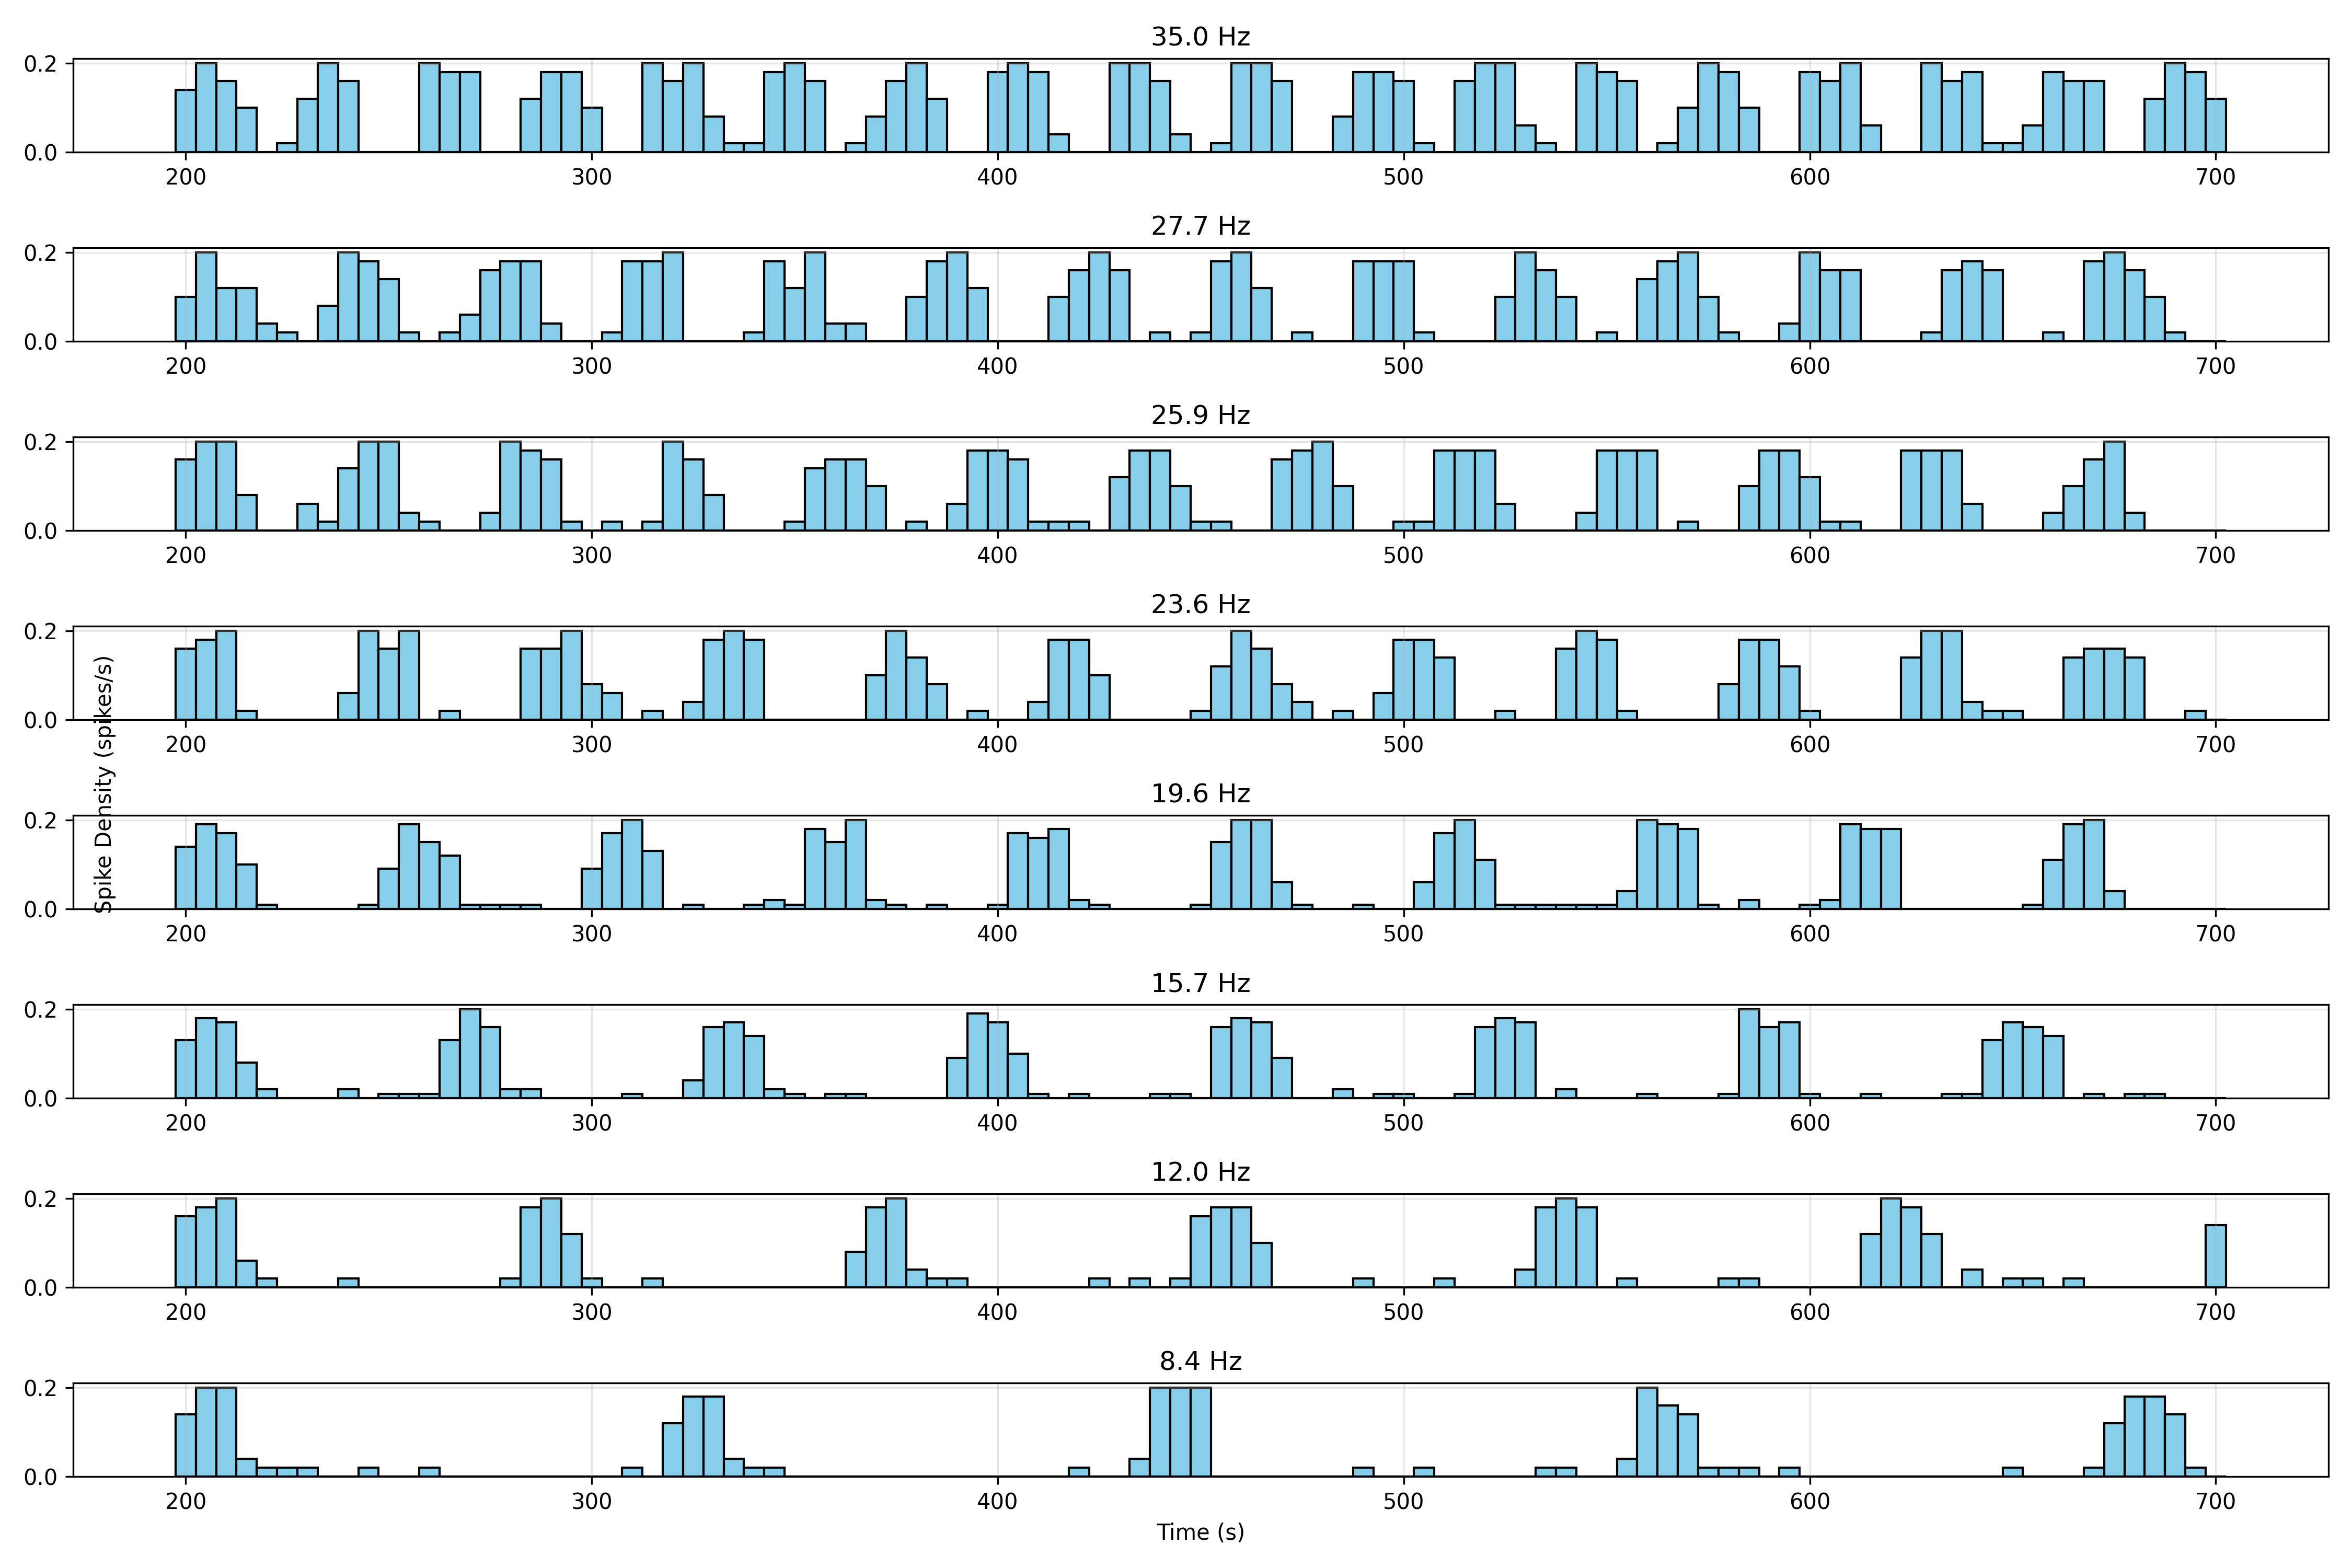
\includegraphics[width=0.9\textwidth]{Fig7.png}
\caption{Spike density during stimulation for all vibratory stimulus frequencies. Each panel represents a different stimulus frequency.}
\label{fig:all_densities}
\end{figure}

The raster plots and spike density histograms clearly show that the recorded neuron in the primary somatosensory cortex exhibits strong, precisely timed responses synchronized to the vibratory stimuli. During stimulation, neuronal firing consistently aligns with each stimulus cycle, especially at higher frequencies (e.g., 27.7 Hz and 35.0 Hz), reflecting robust phase-locking and accurate encoding of the stimulus periodicity. 
This synchronization underscores the neuron's capacity for precise temporal coding and suggests stimulus-driven regularization rather than random background firing.

Additionally, the pronounced sub-Poisson variability supports the conclusion of highly regular and stimulus-dependent firing patterns, pointing to the fact that neuronal and synaptic mechanisms actively contribute to precise timing. 
Overall, these results suggest the neuron reliably encodes tactile vibration frequency through synchronized and sustained spike patterns, critical for sensory perception.

\subsection{Mean and Variance of Spike Count}

The mean and variance of spike counts are calculated during stimulation for all stimulus frequencies and plotted the tuning curve showing the relationship between firing rate and stimulus frequency.




\begin{table}[H]
\centering
\begin{tabular}{ccc}
\toprule
\textbf{Stimulus Frequency (Hz)} & \textbf{Mean Firing Rate (spikes/s)} & \textbf{Variance} \\
\midrule
8.4 & 33.0 & 3.25 \\
11.3 & 39.8 & 2.09 \\
14.2 & 47.2 & 3.84 \\
16.9 & 59.8 & 2.49 \\
23.2 & 71.2 & 6.24 \\
29.0 & 79.0 & 8.65 \\
33.8 & 83.6 & 3.56 \\
35.0 & 105.8 & 11.09 \\
\bottomrule
\end{tabular}
\caption{Mean firing rates and variances for different stimulus frequencies.}
\label{tab:tuning_data}
\end{table}

\begin{figure}[H]
\centering
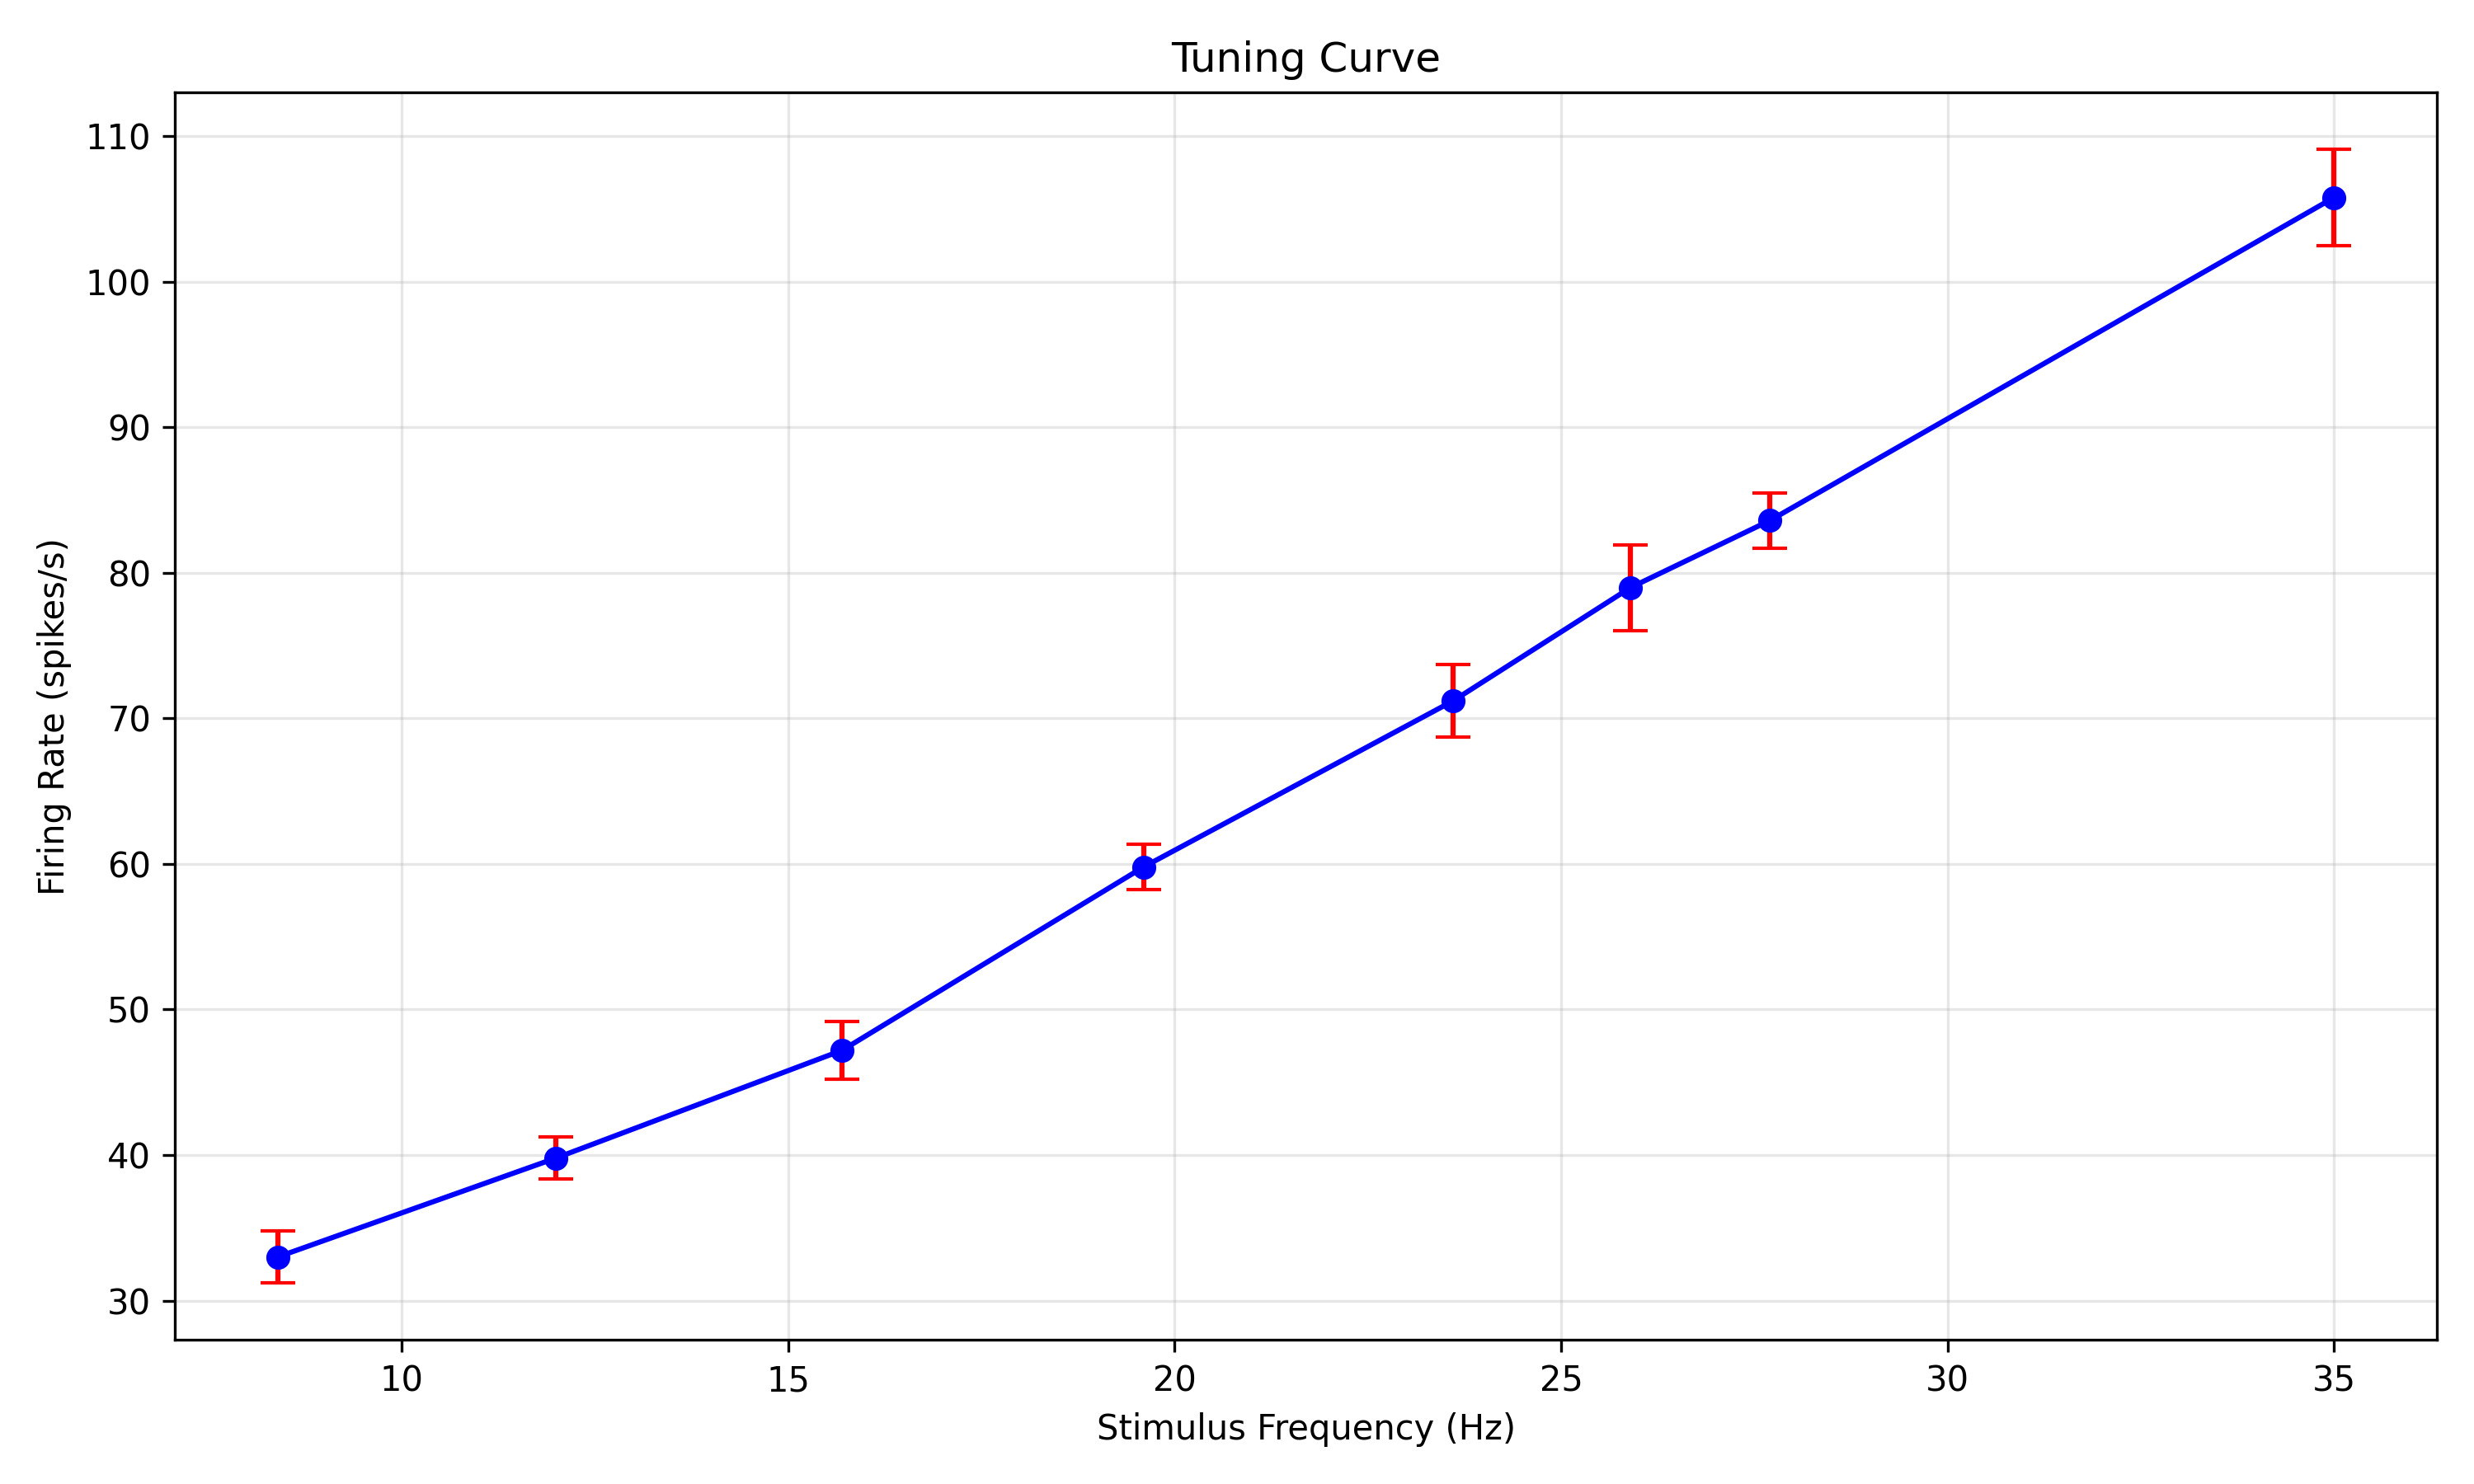
\includegraphics[width=0.7\textwidth]{Fig8.png}
\caption{Tuning curve showing the neuron's mean firing rate during stimulation as a function of stimulus frequency. Error bars represent the standard deviation of spike counts.}
\label{fig:tuning_curve}
\end{figure}

The tuning curve clearly demonstrates that the neuron's mean firing rate consistently increases with stimulus frequency, showing a robust and nearly linear relationship. As the vibratory stimulus frequency rises from approximately 8 Hz to 35 Hz, the neuron's firing rate increases from about 35 spikes/s to over 100 spikes/s. This strong correlation and the small variance observed at each stimulus frequency confirm the neuron’s reliable and precise encoding of tactile stimulus frequency via a rate-coding mechanism, reflecting its capability to distinguish different vibratory frequencies through systematic changes in firing rates.


\section{Conclusion}

The simulations using synthetic Poisson spike trains successfully demonstrated expected statistical properties, including randomness and variability consistent with theoretical predictions. These simulations validated the computational methods used to analyze spike train data.

The analyses performed on actual neuronal data illustrate the neuron's capability to encode vibratory stimulus information robustly through precise temporal and rate-coded mechanisms. The raster plots and spike density functions (Figure 6 and Figure 7) revealed clear phase-locking and regular firing patterns that deviate significantly from pure Poisson statistics, indicative of strong stimulus-driven neuronal synchronization. 

Furthermore, the tuning curve (Figure 8) highlighted a nearly linear relationship between stimulus frequency and firing rate, demonstrating that the neuron reliably distinguishes different tactile vibration frequencies. Collectively, these results reinforce the concept that neurons in sensory cortices employ both temporal precision and firing rate modulation as integral mechanisms for encoding sensory stimuli, contributing crucial insights into neural coding strategies.

\end{document}